\chapter{Quantile regression}
\label{chap:quantreg}

\section{Introduction}
\label{sec:rq-intro}

In Ordinary Least Squares (OLS) regression, the fitted values,
$\hat{y}_i = X_i\hat{\beta}$, represent the \emph{conditional mean} of
the dependent variable---conditional, that is, on the regression
function and the values of the independent variables.  In median
regression, by contrast and as the name implies, fitted values
represent the \emph{conditional median} of the dependent variable.  It
turns out that the principle of estimation for median regression is
easily stated (though not so easily computed), namely, choose
$\hat{\beta}$ so as to minimize the sum of absolute residuals.  Hence
the method is known as Least Absolute Deviations or LAD.  While the OLS
problem has a straightforward analytical solution, LAD is a linear
programming problem.

Quantile regression is a generalization of median regression: the
regression function predicts the conditional $\tau$-quantile of the
dependent variable---for example the first quartile ($\tau = .25$)
or the ninth decile ($\tau = .90$).

If the classical conditions for the validity of OLS are
satisfied---that is, if the error term is independently and
identically distributed, conditional on $X$---then quantile regression
is redundant: all the conditional quantiles of the dependent variable
will march in lockstep with the conditional mean.  Conversely, if
quantile regression reveals that the conditional quantiles behave in a
manner quite distinct from the conditional mean, this suggests that
OLS estimation is problematic.

Gretl has offered quantile regression functionality since version
1.7.5 (in addition to basic LAD regression, which has been available
since early in gretl's history via the \texttt{lad}
command).\footnote{We gratefully acknowledge our borrowing from the
  \texttt{quantreg} package for GNU \textsf{R} (version 4.17).  The
  core of the package is composed of Fortran code written by Roger
  Koenker; this is accompanied by various driver and auxiliary
  functions written in the \textsf{R} language by Koenker and Martin
  M\"achler.  The latter functions have been re-worked in C for gretl.
  We have added some guards against potential numerical problems in
  small samples.}

\section{Basic syntax}

The basic invocation of quantile regression is

\vspace{1em}
\noindent
\qquad \texttt{quantreg} \textsl{tau} \textsl{reglist}
\vspace{1em}

where

\begin{itemize}
\item \textsl{reglist} is a standard \textsf{gretl} regression list
  (dependent variable followed by regressors, including the constant
  if an intercept is wanted); and
\item \textsl{tau} is the desired conditional quantile, in the range
  0.01 to 0.99, given either as a numerical value or the name of a
  pre-defined scalar variable (but see below for a further option).
\end{itemize}

Estimation is via the Frisch--Newton interior point solver
\citep{portnoy97}, which is substantially faster than the
``traditional'' Barrodale--Roberts \citeyearpar{barrodale74} simplex
approach for large problems.

By default, standard errors are computed according to the asymptotic
formula given by \cite{koenker-bassett78}.  Alternatively, if the
\option{robust} option is given, we use the sandwich estimator
developed in \cite{koenker-zhao94}.\footnote{These correspond to the
  \texttt{iid} and \texttt{nid} options in \textsf{R}'s
  \texttt{quantreg} package, respectively.}

\section{Confidence intervals}

An option \option{intervals} is available.  When this is given we
print confidence intervals for the parameter estimates instead of
standard errors.  These intervals are computed using the rank
inversion method and in general they are asymmetrical about the point
estimates---that is, they are not simply ``plus or minus so many
standard errors''.  The specifics of the calculation are inflected by
the \option{robust} option: without this, the intervals are computed
on the assumption of IID errors \citep{koenker94}; with it, they use
the heteroskedasticity-robust estimator developed by
\cite{koenker-machado99}.

By default, 90 percent intervals are produced.  You can change this by
appending a confidence value (expressed as a decimal fraction) to the
intervals option, as in

\vspace{1em}
\noindent
\qquad \texttt{quantreg} \textsl{tau} \textsl{reglist} \verb|--intervals=.95|
\vspace{1em}

When the confidence intervals option is selected, the parameter
estimates are calculated using the Barrodale--Roberts method.  This is
simply because the Frisch--Newton code does not currently support the
calculation of confidence intervals.

Two further details.  First, the mechanisms for generating confidence
intervals for quantile estimates require that the model has at least
two regressors (including the constant).  If the \option{intervals}
option is given for a model containing only one regressor, an error is
flagged.  Second, when a model is estimated in this mode, you can
retrieve the confidence intervals using the accessor \dollar{coeff\_ci}.
This produces a $k \times 2$ matrix, where $k$ is the number of
regressors.  The lower bounds are in the first column, the upper
bounds in the second.  See also section~\ref{sec:bigdata} below.

\section{Multiple quantiles}

As a further option, you can give \textsl{tau} as a matrix---either
the name of a predefined matrix or in numerical form, as in
\verb+{.05, .25, .5, .75, .95}+.  The given model is estimated for all
the $\tau$ values and the results are printed in a special form, as
shown below (in this case the \option{intervals} option was also
given).

{\small
\begin{verbatim}
Model 1: Quantile estimates using the 235 observations 1-235
Dependent variable: foodexp
With 90 percent confidence intervals

      VARIABLE      TAU    COEFFICIENT      LOWER        UPPER

  const             0.05      124.880      98.3021      130.517
                    0.25      95.4835      73.7861      120.098
                    0.50      81.4822      53.2592      114.012
                    0.75      62.3966      32.7449      107.314
                    0.95      64.1040      46.2649      83.5790

  income            0.05     0.343361     0.343327     0.389750
                    0.25     0.474103     0.420330     0.494329
                    0.50     0.560181     0.487022     0.601989
                    0.75     0.644014     0.580155     0.690413
                    0.95     0.709069     0.673900     0.734441
\end{verbatim}
}

The gretl GUI has an entry for Quantile Regression (under
\textsf{/Model/Robust estimation}), and you can select multiple
quantiles there too.  In that context, just give space-separated
numerical values (as per the predefined options, shown in a drop-down
list).  

When you estimate a model in this way most of the standard menu items
in the model window are disabled, but one extra item is
available---graphs showing the $\tau$ sequence for a given coefficient
in comparison with the OLS coefficient.  An example is shown in
Figure~\ref{fig:tau}.  This sort of graph provides a simple means of
judging whether quantile regression is redundant (OLS is fine) or
informative.

In the example shown---based on data on household income and food
expenditure gathered by Ernst Engel (1821--1896)---it seems clear
that simple OLS regression is potentially misleading.  The
``crossing'' of the OLS estimate by the quantile estimates is very
marked.  

\begin{figure}
  \centering
  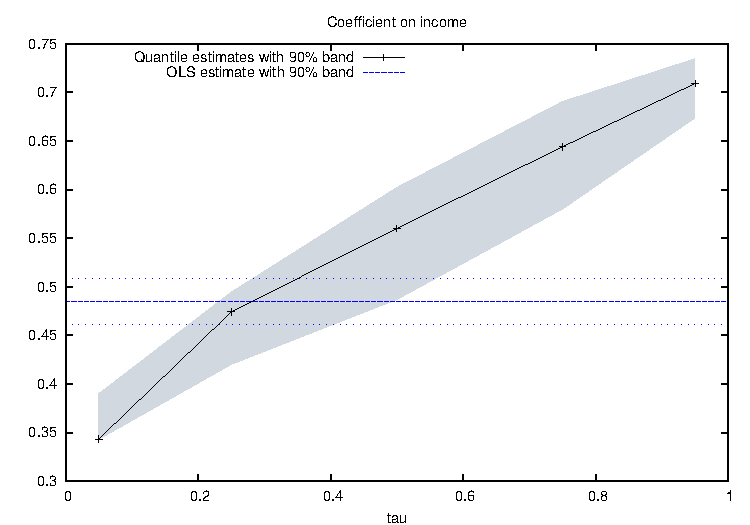
\includegraphics{figures/tau-sequence}
  \caption{Regression of food expenditure on income; Engel's data}
  \label{fig:tau}
\end{figure}

However, it is not always clear what implications should be drawn from
this sort of conflict.  With the Engel data there are two issues to
consider.  First, Engel's famous ``law'' claims an income-elasticity
of food consumption that is less than one, and talk of elasticities
suggests a logarithmic formulation of the model.  Second, there are
two apparently anomalous observations in the data set: household 105
has the third-highest income but unexpectedly low expenditure on food
(as judged from a simple scatter plot), while household 138 (which
also has unexpectedly low food consumption) has much the highest
income, almost twice that of the next highest.

With $n = 235$ it seems reasonable to consider dropping these
observations.  If we do so, and adopt a log--log formulation, we get
the plot shown in Figure~\ref{fig:tau2}.  The quantile estimates still
cross the OLS estimate, but the ``evidence against OLS'' is much less
compelling: the 90 percent confidence bands of the respective
estimates overlap at all the quantiles considered.

\begin{figure}
  \centering
  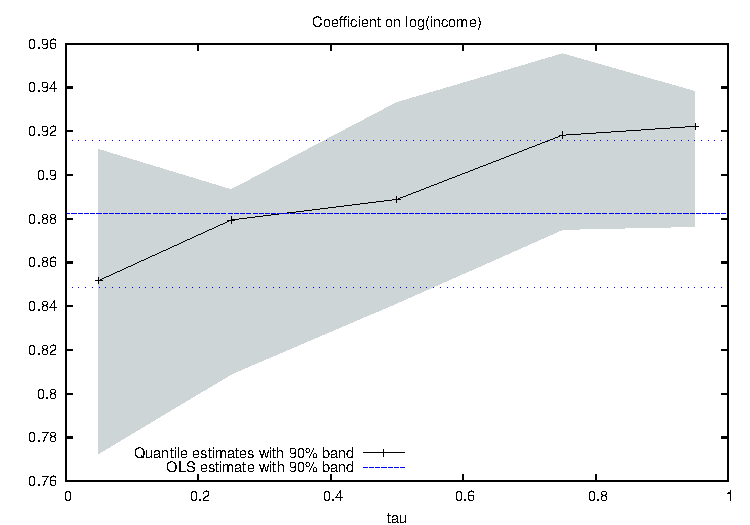
\includegraphics{figures/tau-sequence2}
  \caption{Log--log regression; 2 observations dropped from full Engel data
    set.}
  \label{fig:tau2}
\end{figure}

A script to produce the results discussed above is presented in
listing~\ref{script:engel}.

\begin{script}[htbp]
  \scriptcaption{Food expenditure and income, Engel data}
  \label{script:engel}
\begin{scodebit}
# this data file is supplied with gretl
open engel.gdt

# specify some quantiles
matrix tau = {.05, .25, .5, .75, .95}

# use levels of variables
QM1 <- quantreg tau foodexp 0 income --intervals

# use log-log specification, with two outliers removed
logs foodexp income
smpl obs!=105 && obs!=138 --restrict
QM2 <- quantreg tau l_foodexp 0 l_income --intervals
\end{scodebit}
  The script saves the two models ``as icons''. Double-clicking on a
  model's icon opens a window to display the results, and the Graph
  menu in this window gives access to a tau-sequence plot.
\end{script}

\section{Large datasets}
\label{sec:bigdata}

As noted above, when you give the \option{intervals} option with the
\texttt{quantreg} command, which calls for estimation of confidence
intervals via rank inversion, gretl switches from the default
Frisch--Newton algorithm to the Barrodale--Roberts simplex method.

This is OK for moderately large datasets (up to, say, a few thousand
observations) but on very large problems the simplex algorithm may
become seriously bogged down.  For example, \cite{koenker-hallock01}
present an analysis of the determinants of birth weights, using 
198377 observations and with 15 regressors.  Generating confidence
intervals via Barrodale--Roberts for a single value of $\tau$ took
about half an hour on a Lenovo Thinkpad T60p with 1.83GHz Intel Core 2
processor.

If you want confidence intervals in such cases, you are advised not to
use the \option{intervals} option, but to compute them using the
method of ``plus or minus so many standard errors''.  (One
Frisch--Newton run took about 8 seconds on the same machine, showing
the superiority of the interior point method.)  The script below
illustrates:
%
\begin{code}
quantreg .10 y 0 xlist
scalar crit = qnorm(.95)
matrix ci = $coeff - crit * $stderr
ci = ci~($coeff + crit * $stderr)
print ci
\end{code}
%
The matrix \texttt{ci} will contain the lower and upper bounds of the
(symmetrical) 90 percent confidence intervals.

To avoid a situation where gretl becomes unresponsive for a very
long time we have set the maximum number of iterations for the
Borrodale--Roberts algorithm to the (somewhat arbitrary) value of
1000.  We will experiment further with this, but for the meantime if
you really want to use this method on a large dataset, and don't mind
waiting for the results, you can increase the limit using the
\texttt{set} command with parameter \verb|rq_maxiter|, as in
\begin{code}
set rq_maxiter 5000
\end{code}











